% 
% Tim Sporleder, Manuel Zedel
%
% Ausarbeitung für das Seminar
%	Industrie-Seminar: "Cloud Computing - Wie die Industrie 
%		sich neuen Herausforderungen stellt"
%	von Prof. Dr. Andreas Polze
%	Hasso-Plattner-Institut Potsdam
%	Wintersemester 2014/2015
%
% Basiert auf:
% 	bare_jrnl.tex
% 	V1.4a
% 	2014/09/17
% 	by Michael Shell
%

\documentclass[journal]{IEEEtran}

\usepackage{cite}

\usepackage[pdftex]{graphicx}
\graphicspath{{images/}}
\DeclareGraphicsExtensions{.pdf,.jpeg,.png}

\usepackage[cmex10]{amsmath}
\interdisplaylinepenalty=2500

\usepackage{algorithmic}

\usepackage{array}

\usepackage[caption=false,font=footnotesize]{subfig}

\usepackage{fixltx2e}

\usepackage{url}
\usepackage[utf8]{inputenc} 
\usepackage[ngerman]{babel}

\begin{document}

\title{Vergleich von Cloud-Modellen}

\author{Tim~Sporleder und Manuel~Zedel\thanks{}}

\markboth{Industrie-Seminar: ``Cloud Computing - Wie die Industrie sich neuen Herausforderungen stellt'' 22.03.2015}{}

\maketitle

\begin{abstract}
...
\end{abstract}

\begin{IEEEkeywords}
cloud computing, comparison, deployment models, delivery models
\end{IEEEkeywords}	

\section{Einleitung}
\label{sec_introduction}

\IEEEPARstart{A}{ufgrund} der breiten Verfügbarkeit von Netzwerkinfrastruktur und dem so möglichen Zugang zu IT-Ressourcen über diese Netzwerke wird das Betriebsmodell vieler Systeme geändert. Das Cloud Computing wird laut NIST durch fünf wesentliche Bestandteile definiert - die bereits erwähnte breite Verfügbarkeit von Netzwerkinfrastruktur sowie der Zugriff darauf, die schnelle und einfache Skalierbarkeit der Leistung und Reichweite von Rechenressourcen, das Zusammenfassen von Pools ebendieser Ressourcen die mehreren Nutzern zur Verfügung gestellt werden, sowie die Nutzbarkeit nach dem eigenem Bedarf und schließlich die Verbrauchs-gemäße Abrechnung der Ressourcen.

Dabei wird durch das NIST wie auch im allgemeinen Gebrauch in vier verschiedene Service Modelle im Cloud Computing in Infrastructure as a Service, Platform as a Service und Software as a Service unterteilt. Die Ausprägungen dieser Service Modelle sind jedoch mitunter Anbieter-spezifisch.

Zudem können diese Dienste auf unterschiedliche Weisen abgerufen werden, die Unterscheidung in Private und Public Cloud stellt hierbei eine gebräuchliche Unterteilung dar, auch an diesem Punkt gibt es Anbieter-spezifische Auffassungen bei der Einteilung der bereitgestellten Lösungen. Durch das NIST erfolgt so z.B. neben der Unterscheidung in Private und Public Cloud auch noch die Einteilung in Community und Hybrid Cloud. \cite{nistStandards}

Mit der zunehmenden Anzahl der Anbieter von Cloud Diensten entstehen auch immer neue Möglichkeiten Cloud-Dienste zu kreieren und darauf zuzugreifen. So könnte beispielsweise durch die Möglichkeit dedizierte virtuelle CPUs zu nutzen, die Public Cloud für den Betreiber einer Private Cloud interessanter werden. In dieser Arbeit sollen die speziellen Anforderungen an die jeweilige Serviceform erörtert und daraus resultierende Vorteile beim Betrieb in einer Private, respektive Public, Cloud aufgezeigt werden um eine zeitgemäße Empfehlung bei der Entscheidung für oder gegen das jeweilige Betriebsmodell zu geben. 

Um die verschiedenen Service Modelle genauer zu untersuchen sollen sie zunächst definiert werden und exemplarisch die Unterschiede bei dieser Definition zwischen verschiedenen Herstellern aufgezeigt. Im Anschluss erfolgt die selbige Herangehensweise zur Definition der Eigenschaften von Private und Public Clouds sowie die weiteren Ausprägungsformen der Betriebsmodelle. Auf dieser Grundlage werden die verschiedenen Service Modelle unter Beachtung typischer Einsatzzwecke auf die Möglichkeit der Nutzung im Rahmen der verschiedenen Betriebsmodelle überprüft.
	% manuel

\section{Service Models}
\label{sec_service_models}

\IEEEPARstart{Ü}{blicherweise} wird Cloud Computing als Schichtenmodell (vergl. Figure~\ref{fig:serviceModels}) beschrieben, bei dem Schichten durch die Service Modelle charakterisiert werden. Die unterste Schicht bildet die Infrastruktur der Lösung, bestehend aus der zum Betrieb nötigen Hard- und Software. Die darüber liegende Schicht wird als Plattform bezeichnet, sie besteht für gewöhnlich aus einer Sammlung an Werkzeugen und Diensten mit denen das Programmieren und Bereitstellen neuer Cloudanwendungen vereinfacht und beschleunigt wird. Auf diesen beiden Schichten befindet sich die Software Schicht, mit der Endnutzer in Form von bestehenden Webapplikationen interagieren. \cite{rackSpace}

\begin{figure}
	\centering
	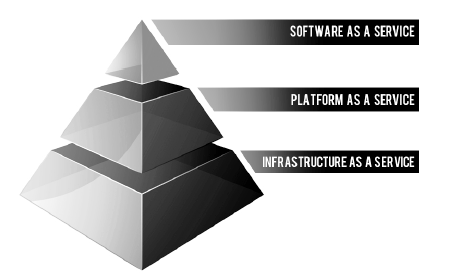
\includegraphics[width=0.95\linewidth]{images/cloudcomputestackimage1}
	\caption{Übersicht Schichten der Servicemodelle}
	\label{fig:serviceModels}
\end{figure}

Auch wenn diese Schichten nicht zusammen genutzt werden müssen, erschließt sich der Zusammenhang jedoch leicht anhand einer Analogie mit der Berliner S-Bahn: Die Schienen bilden die Infrastruktur, die darauf befindlichen Züge stellen die Plattform dar und das S-Bahn Personal, welches die Züge betreibt und so Fahrgäste transportiert dient als Software, welche die ihr zugewiesenen Schienen und Züge nutzt. Im Fall eines Schienenbruchs könnten die Züge auf anderen Strecken zum Einsatz kommen und das Personal könnte auf anderen Verbindungen eingesetzt werden um Fahrgäste zu transportieren.

Dabei gilt es zu beachten, dass die Grenzen zwischen den einzelnen Schichten nicht immer klar gezogen werden können, analog könnte die S-Bahn möglicherweise eine speziell angepasste Antriebstechnik benötigen und so direkt an die Berliner Infrastruktur gekoppelt sein, oder nach der Umstellung auf Draisinen eine der Infrastruktur nähere Betriebsweise eingeführt haben - wodurch der Plattform Charakter in den Hintergrund gerückt werden würde. Als Beispiel einer Infrastruktur die auch gleichzeitig als Plattform fungiert wäre z.B. eine Rolltreppe als Analogie zu betrachten.

Im folgenden Teil der Arbeit werden die verschiedenen Schichten bzw. Service Modelle vorgestellt und auf ebenfalls entstandene Mischformen eingegangen, Tabelle \ref{serviceModelsTable} bildet dabei eine Übersicht über die verschiedenen Modelle.

\begin{figure*}
	\centering
	\begin{tabular}{|l|>{\RaggedRight}p{2cm}|>{\RaggedRight}p{3cm}|>{\RaggedRight}p{3cm}|>{\RaggedRight}p{3cm}|>{\RaggedRight}p{3cm}|}
		\hline
		\rule[-2ex]{0pt}{5.5ex} & \textbf{Paradigmen- wechsel} & \textbf{Merkmale} & \textbf{Vorteile} & \textbf{Nachteile \newline und Risiken} & \textbf{Nicht zu empfehlen bei} \\ 
		\hline
		\rule[-2ex]{0pt}{5.5ex} IaaS & Besitzverhältnis der Infrastruktur & Üblicherweise plattformunabhängig; Infrastruktur-kosten werden geteilt und so reduziert; Service Level Agreements; Nutzungsabhängige Kosten; automatisch skalierend & Kapitalausgaben für Hardware und Betriebspersonal können umgangen werden; ROI Risiken werden verschoben; niedrige Einstiegshürden; optimierte und automatisierte Skalierung & Geschäftsproduktivität und -effizienz hängt stark von den Fähigkeiten des Cloudanbieters ab; potentiell höhere Langzeitkosten; Zentralisierung erfordert neue Sicherheitsmaßnahmen & Größerem Barvermögen als operativem Budget \\ 
		\hline
		\rule[-2ex]{0pt}{5.5ex} PaaS & Lizenzierung & Nutzt Cloud Infrastruktur; eignet sich besonders für agiles Projektmanagement & optimierte Produktveröffentlichung & Zentralisierung erfordert neue Sicherheitsmaßnahmen & - \\ 
		\hline
		\rule[-2ex]{0pt}{5.5ex} SaaS & Besitzverhältnis der Software & Service Level Agreements; Oberfläche meist durch Browser dargestellt; greift auf weitere Cloud Komponenten zu; Kommunikation durch APIs; Zustandslos & Entwicklungskosten können umgangen werden; ROI Risiken werden verschoben; iterative Updates; optimierte Aktualisierung & Zentralisierung der Daten erfordert neue Maßnahmen für die Datensicherheit & - \\ 
		\hline
	\end{tabular}
	\label{serivceModelsTable}
	\caption{Übersicht der Service Arten}
\end{figure*}
 
 
\subsection{Infrastructure as a Service}
Infrastructure as a Service (IaaS) bezeichnet üblicherweise die Bereitstellung von Serverleistung und den dazugehörigen Betriebssystemen, dem Speicherplatz sowie der Netzwerkinfrastruktur. Im Gegensatz zum Kauf der Serverfläche, der Server selber, der Betriebssysteme und deren zugehöriger Software, der zugehörigen Infrastruktur etc. werden hier die benötigten Ressourcen nur nach tatsächlicher Nutzung berechnet.

IaaS stellt für gewöhnlich die Ressourcen ohne Einschränkungen für die Anzahl der Nutzer als Dienst bereit und erlaubt es die bezogene Leistung dynamisch zu skalieren. Mit der Skalierung des genutzten Services wird üblicherweise auch die Berechnungsgrundlage geändert - vergleichbar mit der Berechnung von Strom- oder Gaskosten.

Indem IaaS Anbieter mehr und mehr Konfigurationsunterstützung in Form von Tools und automatisierten Vorgängen bereitstellen, wird die Grenze zur Platform as a Service (PaaS) zunehmend verschoben. Zudem erlauben offene Standards und universell einsetzbare Tools die flexible Kombination von lokal gehosteten Systemen mit denen die durch einen öffentlichen IaaS Anbieter bezogen werden, was als Hybrid Cloud bezeichnet werden kann. \cite{technet}

Aufgrund der weitgehenden Freiheit eines Nutzers bei der Handhabung der genutzten Ressource steht es meist frei Server im Rahmen der Unterstützten Betriebssysteme nach Belieben anzupassen. Im Vergleich zu den noch folgenden Service Modellen Platform- und Software as a Service bietet IaaS damit die höchste Flexibilität und erlaubt z.B. den Einsatz von höchst spezialisierter Software.

Durch die Bereitstellung der bloßen Infrastruktur-Ressourcen beschränkt sich bei diesem Service Modell auch die Service Level Garantie nur auf die Verfügbarkeit der Ressourcen sowie die time to provision einer neuen Einheit. Je nach Ressourcentyp kann dabei jedoch die Garantie für Funktionen die nicht dem Kern des Dienstes entsprechen ausdrücklich verneint werden - so z.B. die Sicherheit der Daten bei einer virtuellen Server Instanz im Vergleich zu der Sicherheit bei einem reinen Cloud Speicheranbieter. Die Verantwortung zur Wahrung solcher Interessen obliegt hier zum größten Teil dem Nutzer. Zudem bedeutet die Nutzung einer nicht eigenen Infrastruktur in der Regel auch eine zunehmende Latenz der errechneten Ergebnisse, sowie einen erhöhten Zeitaufwand beim laden der zu verarbeitenden Daten.

Sinnvoll erscheint die Nutzung von IaaS daher vor allem wenn die dynamische Skalierung der Ressourcen nötig ist, d.h. wenn kurzzeitig eine verstärkte Nachfrage auftritt oder ein plötzlich auftretendes Wachstum der Nutzerbasis eine solche Skalierung verlangt. Zudem ist IaaS für Unternehmen interessant deren Kapitalressourcen nicht ausreichen um die nötige Menge an Hardware zu beschaffen um die für die Geschäftsidee nötigen Systeme zu betreiben. Überdies kann IaaS häufig auch bei Testprojekten oder nur ausgewählten Geschäftsgebieten machen, sodass der Betrieb eines Unternehmens allein auf Basis von IaaS nicht nötig ist.

Von IaaS als Lösung ist jedoch abzuraten wenn die zuvor erwähnten Nachteile überwiegen, d.h. eine sehr große Datensicherheit nötig ist oder die Gesetzeslage es verbietet Daten außerhalb der eigenen Unternehmensgrenzen zu lagern. Auch wenn es sich vor allem um die hochperformante Verarbeitung von großen Datenmengen handelt, die nicht direkt für die auf dem IaaS laufende Anwendung zugänglich ist, ist der zeitliche Mehraufwand beim Datentransfer zu bedenken und eine dedizierte Lösung eventuell besser geeignet. \cite{technet} \cite{rackSpace} \cite{ibm2011}

\subsection{Platform as a Service}
Platform as a Service (PaaS) erweitert die Möglichkeiten des IaaS um Entwicklungsspezifische Punkte, sodass ein PaaS Anbieter für gewöhnlich vorkonfigurierte Entwicklungs- und Laufzeitumgebungen anbietet, die nach Bedarf in der Leistung und Größe skaliert werden können. Wie bei IaaS ist es nicht nötig die Hardware auf der die Software laufen soll zu kaufen, diese wird als Teil des Services gestellt. PaaS Anbieter müssen dank der Möglichkeiten von IaaS nicht einmal selber Infrastruktur besitzen, sondern können sich auf die Optimierung der für ihr PaaS Geschäft nötigen Software konzentrieren. 

Die Leistung einer PaaS besteht dabei jedoch nicht in der Bereitstellung der Software als solches, sondern der Plattform die durch die Software des Anbieters betrieben wird. Üblicherweise bietet ein PaaS Unterstützung für die Entwicklung, das Testen, die Veröffentlichung, den Betrieb sowie die Wartung von Anwendungen in der selben Entwicklungsumgebung. Der Zugriff auf die Umgebung ist dabei multi-tenant fähig, sodass speziell agile Entwicklungsmethoden mit verteilten Entwicklerteams unterstützt werden. 

Die Entwicklungsunterstützung kann dabei in Form von vordefinierten UI Elementen, vorkonfiguriertem Load-Balancing und Skalierungsmaßnahmen bis hin zur Integration mit anderen Webdiensten, Datenbank und Hardware erfolgen. Aufgrund der zunehmenden Verbreitung von Standards in der Entwicklung ist es zudem leicht möglich diese vordefinierten Funktionen zu erweitern. 

Meistens unterscheiden sich die verschiedenen Plattformen im Ausmaß der Vorarbeit bzw. der Konfigurierbarkeit, diese kann von der Entwicklungsumgebungen reichen, bei denen allein die Laufzeitumgebung sowie die Kontrolle über die Leistungsfähigkeit der angeforderten Instanz gegeben wird bis hin zu vorkonfigurierten, komplexen UI Elementen zur Verarbeitung von bereitgestellten Daten, mit denen ohne Programmieraufwand eine Anwendung entwickelt werden kann.

Aufgrund des Fokus' auf die Entwicklungsunterstützung bietet PaaS auch hier den größten Vorteil, da komplexe IT Anwendungen häufig von komplexen Entwicklungsstrukturen begleitet werden. Damit einher gehend ist die Nutzung von PaaS ebenfalls für Entwicklungen mit automatisierten Tests und häufigen Iterationen zu empfehlen, da der hohe Automatisierungsgrad eine ständige Neuinstallation stark vereinfacht und somit die dabei auftretenden Probleme von Beginn an behandelt werden können.

Allerdings gilt es bei PaaS den Einsatzzweck auf die Nutzbarkeit mit einem PaaS zu überprüfen sowie bei der vom PaaS verwandten Technologie darauf zu achten ob man einem Vendor lock-in entgehen könnte. Wie auch bei IaaS ist auch hier die Performancebetrachtung wichtig, da die standardisierten Umgebungen wenig Spielraum zulassen, spezielle Betriebssystemfunktionen oder Fremdsoftware zu nutzen bzw. anzupassen, im Gegensatz zu IaaS gilt diese Limitierung auch beim Betrieb einer eigenen PaaS Umgebung. \cite{technet} \cite{rackSpace} \cite{ibm2011}

\subsection{Software as a Service}
Software as a Service (SaaS) bildet die oberste Schicht in der schichtweisen Betrachtung des Cloud Computing und wird so auch häufig durch die Nutzung einer der beiden darunter liegenden Schichten realisiert. Im Vergleich zu den vorherigen Modellen ist die so angebotene Software von den darunter befindlichen Strukturen abstrahiert und für Endnutzer zugänglich. Software die als SaaS angeboten wird, kann vom Nutzer über ein Netzwerk genutzt werden und verlangt so keine Installation. Diese Auslieferungsmethode bringt zudem den Vorteil, dass Nutzer sich nicht mehr um die Wartung der Software kümmern müssen und bei der Entwicklung von einer deutlich geringeren Versionsfragmentierung ausgegangen werden kann. Wie auch bei den vorangegangenen Schichten wird die SaaS Schicht durch APIs erweiterbar gehalten und nutzt für gewöhnlich fremde APIs um realisiert zu werden.

Vor allem durch den hohen Grad an Standardisierung der Software bietet sich die Nutzung von SaaS für grundlegende Softwaresysteme an, die nicht zum Kernbereich des jeweiligen Unternehmens zählen, email- sowie CRM-Systeme stellen hier ein gängiges Beispiel für den SaaS Einsatz dar. Derartige Systeme sind typischerweise für den laufenden Betrieb eines Unternehmens wichtig, bieten jedoch selten einen großen Wettbewerbsvorteil bei eigenen Anpassungen. Durch die Vereinbarung von Service Level Agreements ist es vor allem möglich eine gute Erreichbarkeit der Lösung zu gewährleisten - üblicherweise liegt die zugesicherte Erreichbarkeit der Systeme bei 99\% und höher. Auch hier werden derartige Dienste entsprechend der Nutzungsdauer bezahlt.

Die leichten Skalierungsmöglichkeiten der einer SaaS Lösung zugrunde liegenden Cloud Infrastruktur erweist sich als weiterer Indikator auf den Einsatz einer solchen Lösung zu setzen. Ist es zu erwarten, dass die Software nur über kurze Zeiträume unter hoher Last stehen wird, wie z.B. bei Verkaufssystemen vor Weihnachten oder zu Beginn eines neuen Jahres. Auch wenn die Nutzung der Software nur für einen begrenzten Zeitraum benötigt wird, bietet sich die Verwendung von SaaS an. Ebenso kann das über ein Netzwerk erfolgende Angebot der Software ausgenutzt werden, da Anwendungen mit einem hohen Grad an Interaktion mit anderen Systemen leichter mit diesen sowie weiteren Diensten kommunizieren können. Mit Blick auf die zunehmende Verbreitung der mobilen Internet Nutzung sowie der verbreiteten Unterstützung verschiedener Anzeigegrößen im SaaS Umfeld, ist der Einsatz einer SaaS Lösung auch von Interesse wenn ein möglichst nahtloser Übergang zwischen verschiedenen Gerätetypen gewährleistet werden soll, da die SaaS-Anwendung die selbe bleibt und so z.B. keine Brüche im Datenbestand auftreten. Nicht zuletzt ist eine SaaS Lösung zu empfehlen wenn die Versionsfragmentierung minimal gehalten werden soll.

Im Gegenzug bietet sich eine SaaS Lösung nicht an wenn die benötigte Funktion bereits durch eine existierende on-premise abgedeckt wird, d.h. bestehende Systeme durch eine SaaS Einführung nicht weiter genutzt werden würden. Ebenso stellt, wie auch bei der IaaS, die Gesetzgebung oder die Firmengrundsätze eine Entscheidungsgrundlage dar, ist vor allem bei einer öffentlichen SaaS Lösung nicht auszuschließen, dass Daten das Land oder das Firmennetzwerk verlassen. Und ebenfalls wie bei der IaaS zutreffend ist auch bei SaaS die nötige Verarbeitungsgeschwindigkeit entscheidend, die sofortige Verarbeitung anfallender Echtzeitdaten kann bei SaaS nicht immer gewährleistet sein und so eine on-premise Lösung erstrebenswerter machen. \cite{technet} \cite{rackSpace} \cite{ibm2011}

\subsection{Everything as a Service}
Neben den hier aufgeführten Modellen wird das Servicemodell auch in anderen Formen in Verbindung zum Cloud Computing gebracht, so gibt es die Möglichkeit Business Process as a Service zu nutzen um z.B. weitere Teile des Tagesgeschäfts automatisieren zu können, zudem werden auch die eventuell nötigen Schritte zur Skalierung oder zum Start einer Cloudlösung angeboten und als Cloudsetup as a Service vertrieben. Der Computing Aspekt ist dabei weit weniger im Vordergrund als bei den vorangegangenen Modellen. Überdies gibt es Spezialisierungen der Modelle, sodass der Betrieb angepasster Datenbanken als Database as a Service betrieben wird oder Plattformen die mit minimalem Aufwand zur vollständigen Software as a Service aufgebaut werden können, wofür Wordpress as a Service beispielhaft ist.

\section{Private vs. Public}
\label{sec_privacy_models}

\IEEEPARstart{U}{nabhängig} von der Serviceform erfolgt die Einteilung zudem nach der Art der Bereitstellung eines Clouddienstes. Dabei richtet sich die Unterscheidung nach dem Eigentumsverhältnis der zugrundeliegenden Systeme und dem damit verbundenen Grad an Anpassbarkeit. Die Anpassbarkeit bezieht sich dabei sowohl auf die Architektur als auch auf die des jeweiligen Dienstes. 

Aus diesen Unterscheidungen ergeben sich ferner weitere Charakteristiken der einzelnen Bereitstellungsmodelle - dargestellt in Tabelle \ref{deploymentTypesTable}. Abhängig von der Bereitstellung variieren die Kosten, die Kontrollmöglichkeit und die Skalierbarkeit.

\begin{figure*}
	\begin{tabular}{|>{\RaggedRight}p{3cm}|>{\RaggedRight}p{1.6cm}|>{\RaggedRight}p{2.2cm}|>{\RaggedRight}p{2.5cm}|>{\RaggedRight}p{2.7cm}|>{\RaggedRight}p{3cm}|}
		\hline
		\rule[-2ex]{0pt}{5.5ex} \textbf{Art der \newline  Bereitstellung} & \textbf{Hosting} & \textbf{Geteilt oder Dediziert} & \textbf{Kontrolle über Architektur} & \textbf{Skalierbarkeit} & \textbf{Art der Investition} \\ 
		\hline
		\rule[-2ex]{0pt}{5.5ex} Shared Public & Extern & geteilt & Cloudanbieter oder Markt & minimale Einschränkungen & Nutzungsabhängig \\ 
		\hline
		\rule[-2ex]{0pt}{5.5ex} Dedicated Public & Extern & (Teilweise) dediziert & Cloudanbieter oder Markt & Vertragsabhängig & Nutzungsabhängig \\ 
		\hline
		\rule[-2ex]{0pt}{5.5ex} Self Hosted Private & Intern & Dediziert & Voll & Investitionsabhängig & Cloud-Aufbau, ROI durch Serviceangebot \\ 
		\hline
		\rule[-2ex]{0pt}{5.5ex} Hosted Private & Extern & Dediziert & Voll & Vertrags- oder Investitionsabhängig & Vertragsabhängig, möglicherweise mit Auswirkung auf Barvermögen \\ 
		\hline \rule[-2ex]{0pt}{5.5ex} Private Appliance & Intern & Dediziert & Cloudanbieter & Angebotsabhängig & Vertragsabhängig, möglicherweise mit Auswirkung auf Barvermögen \\ 
		\hline 
	\end{tabular}
	\centering
	\caption{Deployment Arten Übersicht}
	\label{deploymentTypesTable}
\end{figure*}

\subsection{Public Cloud}
Anbieter von IT Ressourcen als SaaS, PaaS und speziell als IaaS müssen die Rechenleistung in Form von Rechenzentren bereitstellen, um die Verfügbarkeit dieser Ressourcen über weite Strecken zu gewährleisten, erfolgt dies in der Regel über Orts- und Ländergrenzen hinweg. Im Fall einer public Cloud befindet sich die zugrundeliegende Schicht im Eigentum des jeweiligen Cloud Anbieters.

Diese Ressourcen werden mehreren Kunden zur Verfügung gestellt, was zu einer Kostenreduktion für den einzelnen Nutzer führt und die vorhandenen Kapazitäten besser ausnutzt - z.b. indem die nicht benötigte Leistung eines Kunden sinnvoll mit dem Abfangen eines hohen Leistungsbedarfs eines anderen Kunden kombiniert werden kann.
Im Gegenzug bedeutet diese Ressourcenteilung jedoch z.B. auch die gemeinsame Nutzung von Speicher bzw. die geringere Kontrolle über die eingesetzte Software und die so verarbeiteten Daten.

Die vorgestellten Service Modelle (IaaS, PaaS und SaaS) sind alle sowohl als private als auch als public Lösung zu finden.

Auch das Angebot der Public Cloud bietet weitere Unterscheidungsmöglichkeiten in Bezug auf die Hosting Form.

\subsubsection{Shared Public Cloud}
Wird der Service auf einer mit mehreren Benutzern geteilten Schicht betrieben, deren Architektur, Absicherung und Verwaltung durch den Anbieter erfolgt, wird von einer Shared Public Cloud gesprochen. Auch die Anpassbarkeit wird hier durch den Anbieter vorgegeben. Durch diese Bedingungen ist es möglich besonders günstige Kosten für den Betrieb zu veranschlagen und den Umfang der Serviceleistung nach Bedarf zu skalieren. 

\subsubsection{Dedicated Public Cloud/ Virtual Private Cloud}
Das direkte Gegenstück zur Shared Public Cloud bildet die Dedicated Public Cloud, bei der ein Teil der Ressourcen der Shared Public Cloud einem Kunden dediziert zur Verfügung gestellt werden. Durch den Ausschluss weiterer Nutzer der selben Infrastruktur bietet sich häufig eine bessere Leistungsfähigkeit als bei der Shared Public Cloud, ebenso können meist mehr Sicherheitsmaßnahmen getroffen werden und anderweitige Anpassungen des Dienstes vorgenommen werden. Auch wenn es sich um dedizierte Systeme handelt, erfolgt das Hosting der Dienste auf Systemen im Besitz des Anbieters.

\subsection{Private Cloud}
Die IT Ressourcen werden bei einer Private Cloud exklusiv für einen Kunden bereitgestellt. Damit können Anforderungen an Sicherheit, Privatsphäre im hohen Maß erfüllt werden und das Vertrauen in die Cloud Lösung erhöht werden. Dazu bietet eine derartige Lösung die Möglichkeit innerhalb des zur Verfügung stehenden Vorrats an Ressourcen nach Bedarf zu skalieren und diese Ressourcen so bestmöglich zu nutzen.

Die Verwendung einer privaten Cloud Lösung bietet sich vor allem an, wenn das Gesetzes- oder Unternehmensumfeld strenge Vorgaben an den Betrieb der IT stellt oder das Vertrauen in einen passenden Cloudanbieter nicht ausreicht um die nötige Lösung in dessen Public Cloud zu hosten. 

Wie auch bei der Public Cloud kann die Private Cloud anhand der Hosting Form unterschieden werden.

\subsubsection{Self-Hosted Private Cloud}
Die Self-Hosted Private Cloud stellt auf Basis der bestehenden Systeme und Services eine im Rahmen dieser skalierbare Cloud Umgebung. Dadurch behält man die volle Kontrolle über die Systeme, kann die Architektur nach Belieben anpassen und die Auslastung der Systeme maximieren.

\subsubsection{Hosted Private Cloud}
Im Vergleich zur Dedicated Public Cloud/ Virtual Private Cloud, ist die Hosted Private Cloud zwar ebenfalls im Data-Center eines Cloudanbieters angesiedelt und wird mittels der Dienste dieses Anbieters betrieben, allerdings können die dazu nötigen Systeme vom Kunden angepasst werden und werden durch den Kunden dediziert gemietet. Durch diese Konstellation lässt sich der Vorteil einer in einem Data-Center befindlichen Lösung mit der Kontrolle wie bei einer Self-Hosted Private Cloud kombinieren.

\subsubsection{Private Cloud Appliance}
Bei einer Private Cloud Appliance wird eine von einem Cloudanbieter entworfene und angepasste Cloudumgebung beim Kunden installiert und durch diesen oder den Cloudanbieter selbst gewartet. Dadurch ist es möglich die Interoperabilität der Dienste des Cloudanbieters nutzen zu können ohne die Sicherheit oder die Kontrolle über die Daten einzuschränken, allerdings ist die Skalierung meist nur im Rahmen der vorhandenen Umgebung möglich.

\subsection{Hybrid Cloud}
Neben der Unterscheidung in Private- und Public Cloud ergibt sich auch ein Raum für Mischformen, bei denen verschiedene Cloud Infrastrukturformen miteinander kombiniert werden. Die Komposition erfolgt dabei so, dass die Teilbestandteile eigenständig funktionieren, bei Bedarf jedoch zwischen den Bestandteilen ausgetauscht werden kann um z.B. Lastspitzen abzufangen oder um Teilberechnungen auf einem angepassten Dienst durchzuführen. Als Hybrid Cloud werden auch Systeme bezeichnet, die verschiedene Dienste der gleichen Infrastrukturform komponieren wie z.B. mehrere Public Cloud Dienste.

Besonders bietet sich diese Form an, wenn datenschutzkritische Prozesse gesondert in einer Private Cloud und datenschutzunkritische Prozesse in einer Public Cloud bearbeitet werden können, da so die Einspar- sowie Skalierungsmöglichkeiten der Public Cloud genutzt werden und gleichzeitig die Datenexposition verhindert werden kann. Die Unterteilung von Geschäftsprozessen in diese Kategorien stellt dabei jedoch keine geringe Hürde dar. \cite{technet}		% manuel

\section{SAP}
\label{sec_sap}

\IEEEPARstart{S}{AP}...			% tim

\section{Fujitsu}
\label{sec_fujitsu}

\IEEEPARstart{F}{ujitsu}...

\subsection{Cloud und Fujitsu}
\label{sec_fujitsu_general}



\subsection{Service-Modelle}
\label{sec_fujitsu_delivery}



\subsection{Betriebsmodelle}
\label{sec_fujitsu_deployment}

		% tim

\section{Amazon}
\label{sec_amazon}

\IEEEPARstart{A}{mazon} hat um eine der größten online Verkaufsplattformen der Welt betreiben zu können eine stetig wachsende Infrastruktur geschaffen. Aus der dafür entwickelten Basis zur bedarfsgerechten Nutzung von Rechen- und Speicherressourcen sowie deren Management entstanden die Amazon Web Services. Mit Hilfe dieser Dienste ist es möglich Systemressourcen für die Entwicklung schnell abzurufen.

\subsection{Cloud und Amazon}
\label{sec_amazon_general}
Die Amazon Web Services stellen aufgrund der Vielfalt an Diensten, der Preisgestaltung sowie der Integration der Dienste untereinander einen Marktführer im Bereich Cloud Computing dar. Die Produkte zum Management der Daten und Cloudinstanzen entstammen dabei der internen Nutzung Amazons, so z.B. die DynamoDB als Datenbank für große Datenmengen mit vorhersagbaren Zugriffszeiten, die ihren Ursprung in der Datenhaltung der Artikeldaten für den Amazon Onlinehandel hat oder EC2, der Dienst um virtuelle Server anzufordern, der zunächst in der internen Produktentwicklung für Amazon zum Einsatz kam.

Um die entstandenen Dienste der Allgemeinheit zugänglich zu machen und so die vorhandene Infrastruktur besser ausnutzen zu können wurden die Dienste als Teil des public Cloud Angebots verfügbar gemacht.

\subsection{Service-Modelle}
\label{sec_amazon_delivery}
Die in Abbildung \ref{fig:amazon} dargestellten Dienste zeigen die Reichweite der angebotenen Services, dabei wird ersichtlich, dass neben den verschiedenen Zusatzdiensten der IaaS Bereich der Cloudanwendungen die größte Abdeckung bietet. Die IaaS sowie PaaS Angebote entstammen dabei vorwiegend dem Eigenbedarf an Lösungen und wurden mit fortschreitender Entwicklung für die public Cloud angepasst. Die Vertriebsplattform Amazon wird demnach auf Grundlage ebendieser Dienste betrieben.

Die SaaS Lösungen des Unternehmens sind im Vergleich zu den übrigen Kategorien die jüngsten, wurde mit Amazon WorkMail erst 2015 der auf Unternehmen abzielende E-Maildienst von Amazon vorgestellt.

\begin{figure*}
	\centering
	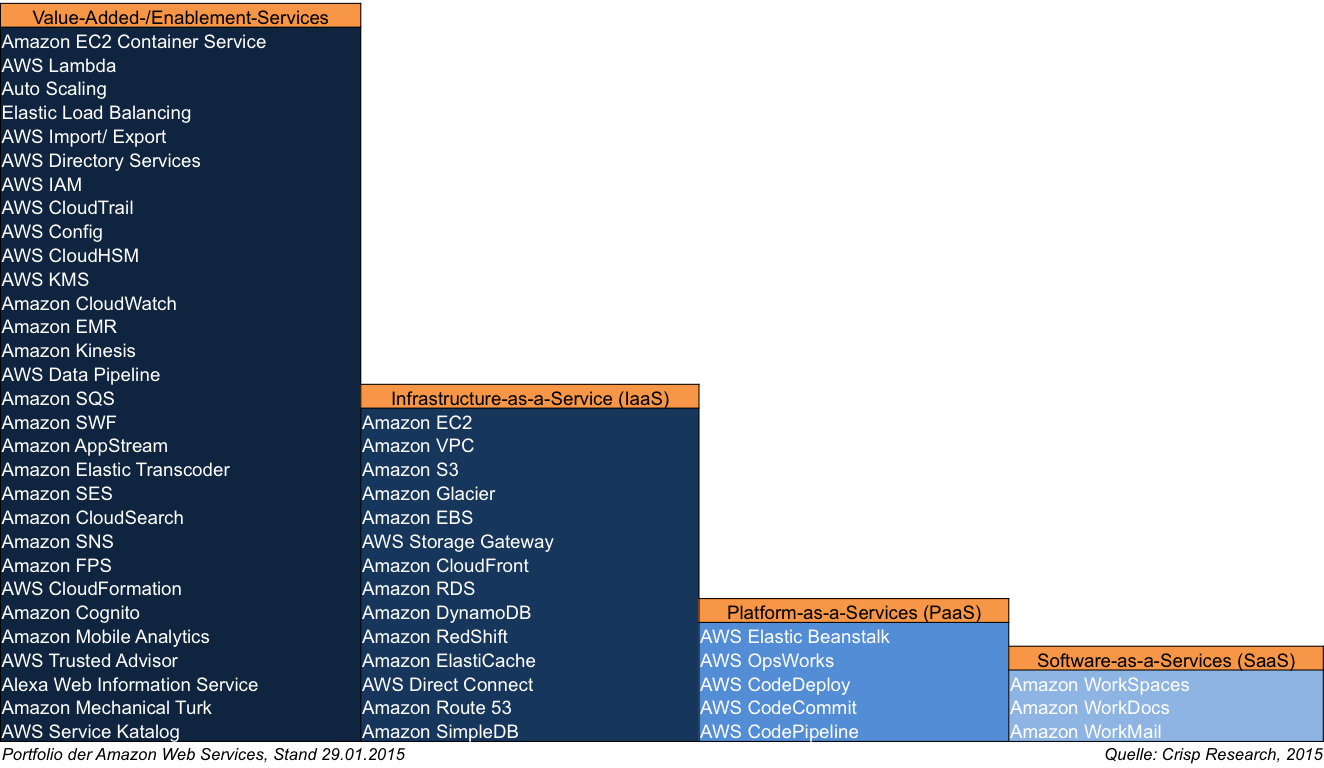
\includegraphics[width=0.8\linewidth]{images/Crisp-AWS-Portfolio_201501291}
	\caption{Amazon Web Services Portfolio}
	\label{fig:amazon}
\end{figure*}

\subsection{Betriebsmodelle}
\label{sec_amazon_deployment}
Die unterschiedlichen Cloud Dienste werden von Amazon als Teil ihres public Cloud Angebots betrieben und in der Regel als Shared Public Cloud angeboten.

Amazon bietet jedoch auch die Möglichkeit eine Dedicated Public Cloud zu betreiben, dieses wird als "Amazon Virtual Private Cloud (Amazon VPC)" bezeichnet. Dabei gilt es allerdings zu beachten, dass es sich nur um virtuell private Server handelt, was es zwar erlaubt virtuelle Netzwerke von selbst konfigurierten  Systemen erstellen zu können, diese jedoch die darunterliegende Hardware mit anderen Anwendungen teilen. 

Eine Möglichkeit eine Private Appliance, Self Hosted Private oder Hosted Private Cloud mit den Mitteln der Amazon Web Services zu betreiben gibt es nicht.		% manuel

\section{Stand der Technik}
\label{sec_facts}

\IEEEPARstart{A}{ufgrund} der fehlenden Standards beim Aufbau der Cloudinfrastruktur und dem damit verbundenen Bestreben der unterschiedlichen Anbieter die eigenen Kunden durch angepasste Techniken an sich zu binden, ist es heute noch nicht überall möglich Cloudanwendungen über Anbietergrenzen hinweg zu verschieben. Die Interoperabilität - vor allem von public Cloudservices - ist dabei jedoch meist gewährleistet, da die Integration einzelner Anwendungen mit weiteren Diensten eine typische Eigenschaft des Cloud Computing darstellt.

Idealerweise ist es möglich eine lokal ausgeführte Instanz eines Dienstes in die Umgebung eines Cloudanbieters zu verschieben, je nach Cloudanbieter ausgehend z.B. von Images virtueller Maschinen oder plattformabhängigem Quellcode. Da nicht von einer einzigen Cloud auszugehen ist, wäre so auch die Möglichkeit gegeben über Anbietergrenzen hinweg zu skalieren indem zusätzliche Instanzen bei anderen Cloudanbietern gestartet werden oder zwischen Anbietern gewechselt wird.

Allerdings ermöglicht der Einsatz neuer Technologien einen höheren Grad an Flexibilität beim Betrieb von Cloudanwendungen. Ermöglicht wird dies etwa durch die Unterstützung transportabler Container oder die Entwicklung von abstraktionsabhängig standardisierten Schnittstellen.

\subsection{Interoperabilität und Portabilität}
Interoperabilität und Portabilität in der Cloud bezieht sich auf die Möglichkeit bestehende, wiederverwendbare Komponenten der verschiedenen Servicearten zu Systemen zu kombinieren.

Die Portabilität bezieht sich dabei auf die Daten um bestehende Daten in verschiedenen Anwendungen nutzen zu können, auf Anwendungen um diese bei unterschiedlichen PaaS auszuführen und auf Plattformen welche es erlauben durch erneute Kompilierung oder die Migration bestehender Images virtueller Maschinen zwischen Cloudanbietern zu wechseln.

Hingegen bezeichnet die Interoperabilität die Grundlage für Anwendungen miteinander zu kommunizieren. Ein wichtiger Aspekt dabei liegt in der Möglichkeit Daten synchron halten zu können sowie in der Kommunikation z.B. in einer Hybrid Cloud, um hohe Auslastungen abfangen zu können.
Die Interoperabilität ist zudem auf Plattformebene nötig um einzelne Anwendungskomponenten über Plattformgrenzen hinweg miteinander interagieren zu lassen.
Aufgrund der zunehmenden Anzahl an Marktplätzen für Cloudanwendungen und PaaS Umgebungen wird auch eine Interoperabilität zwischen diesen Veröffentlichungs- und Bezugspunkten erstrebt um die Produkte leichter für den Nutzer zugänglich zu machen.

Um die Vorzüge des Cloud Computing von leicht zugänglichen Ressourcen, vergleichbar mit der Nutzung von Elektrizität und Wasser zu gewährleisten ist es wichtig diese Funktionen zu bieten um den Integrationsaufwand sowie die Mehrkosten für den Einsatz neuer Anwendungen gering zu halten.

\begin{figure*}
	\centering
	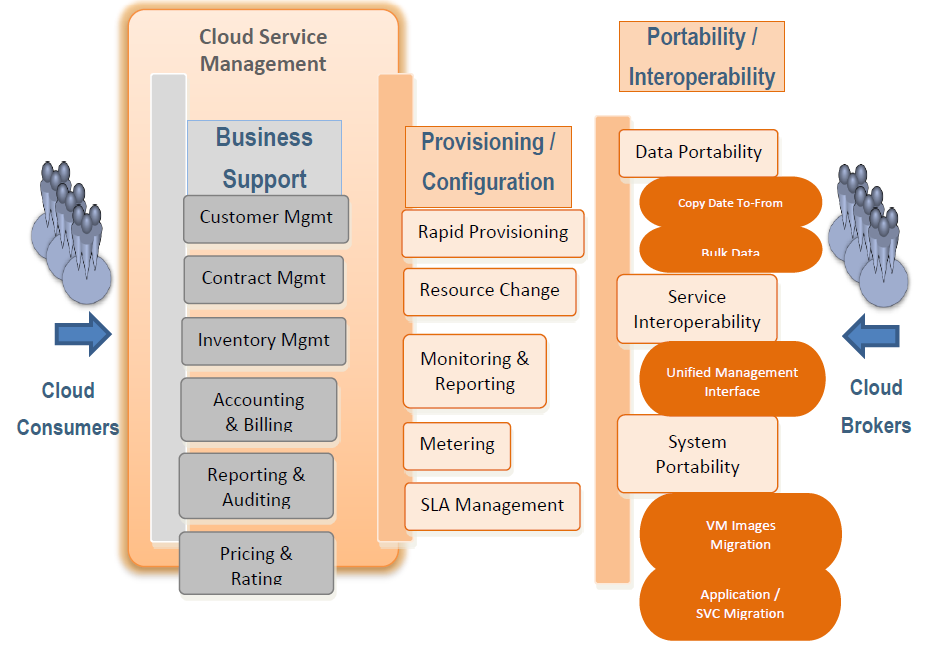
\includegraphics[width=0.8\linewidth]{images/portability}
	\caption{Schematischer Vergleich virtuelle Maschine und Container}
	\label{fig:portability}
\end{figure*}

\subsection{OpenStack}
Unter der Bezeichnung OpenStack wird eine Plattform entwickelt, die es ermöglicht eine IaaS oder PaaS Lösung zu betreiben. Die zu OpenStack gehörigen Projekte stellen jeweils Teilaspekte des Betriebs einer Cloud Computing Lösung sicher. Die Verwaltung mehrerer virtueller Maschinen wird so z.B. durch OpenStack Compute (Nova) ermöglicht, die Verwaltung erfolgt über OpenStack Dashboard (Horizon), welches eine übersichtliche Darstellung und Konfiguration der OpenStack Plattform ermöglichen soll oder der OpenStack Database Service - Trove genannt - durch den Datenbanken als Dienst zur Verfügung gestellt werden sollen. Auch das Heat genannte Orchestrierungswerkzeug, mit dessen Hilfe Konfigurationen ("Stacks") zur automatisierten Bereitstellung und Skalierung einer ganzen Cloud-Infrastruktur realisiert werden kann, ist Teil von OpenStack.

OpenStack wurde 2010 von RackSpace Hosting zusammen mit der NASA begründet und wird mittlerweile von zahlreichen Unternehmen unterstützt, neben RackSpace zählen auch Hewlett-Packard, IBM und VMware zu den Unterstützern. Die Marktführer Amazon, Google und Microsoft zählen hingegen nicht zu den Unterstützern, die APIs der OpenStack Äquivalente zum Amazon EC2 und Amazon S3 Dienst sind jedoch kompatibel, sodass eine Portierung bestehender Anwendungen leicht möglich ist. Aufgrund der breiten Verfügbarkeit der OpenStack Ressourcen ist es möglich eigene (private) Cloud-Infrastrukturen zu erstellen und diese in die Cloud eines Cloud-Anbieters zu verschieben.

Die verschiedenen Services decken so die Bereitstellung speziell der IaaS sowie der PaaS Schicht ab.

\subsection{Docker}
Docker bietet eine Möglichkeit einen der Kritikpunkte bei der Nutzung von virtuellen Maschinen zu umgehen, indem es die Ausführung von Prozessen in vom Betriebssystem verwalteten Containern ermöglicht bzw. vereinfacht.

Während bei virtuellen Maschinen ein gesamtes Betriebssystem betrieben und von weiteren virtualisierten Instanzen getrennt wird, wird beim Einsatz von Containern nur der Prozess in einer virtualisierten Umgebung betrieben, sodass mehrere Container sich ein Hostsystem "teilen" können und dennoch voneinander getrennt auf die Ressourcen zugreifen (vergl. Abbildung \ref{fig:docker}). Die Handhabung der Container wird dabei von Linux' LXC übernommen. Überdies ermöglicht Docker auch das Erstellen und Veröffentlichen von Containern, sowie die Orchestrierung mehrerer Container einer Anwendung. Teilweise ergibt sich eine Überlappung der Möglichkeiten von OpenStack und Docker, da Docker ebenfalls in der Lage ist Images, Systemkonfigurationen oder fertige Cloudanwendungen zu erstellen und zu verwalten und es überdies z.B. auch vergleichbare Dashboard Lösungen für Docker gibt. Allerdings profitiert Docker von der Unterstützung und Verbreitung von OpenStack, da es sich gut mit OpenStack Nova integrieren lässt.

Ferner erlaubt es Docker Container über Anbietergrenzen hinweg zu verschieben und neue Anwendungsinstanzen in Containern bei unterschiedlichen Cloud-Anbietern zu starten. Die Unterstützung, vor allem durch Amazon, Google sowie Microsoft ermöglicht so tatsächliche Interoperabilität innerhalb des Cloudangebots.

\begin{figure*}
	\centering
	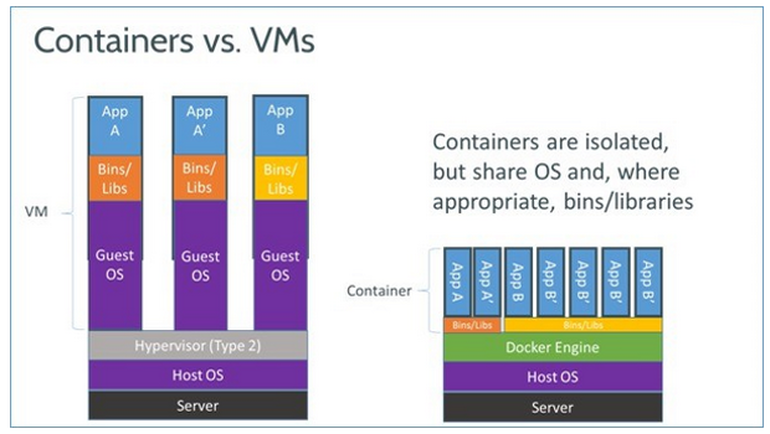
\includegraphics[width=0.8\linewidth]{images/docker-vm-container}
	\caption{Schematischer Vergleich virtuelle Maschine und Container}
	\label{fig:docker}
\end{figure*}

\section{Stand der Implementierungen}
\label{sec_implementations}
Die Cloud Computing Implementierungen in Unternehmen werden von Marktanalysten ständig überwacht und der Erfolg von Unternehmen wie Instagram, die ohne eigener Infrastruktur eine enorme Nutzerzahl erreichen konnten gibt Anlass eigene Anwendungen in die Cloud zu portieren. Dabei ergibt sich jedoch die Herausforderung, wie die zur Verfügung stehenden Möglichkeiten im Einzelfall genutzt werden können. Im allgemeinen unterscheidet sich die Herangehensweise mit Blick auf die bestehenden Systeme bzw. die Möglichkeit Neuentwicklungen zu tätigen.

\subsection{Verbreitung bei Neuentwicklungen}
Bei neuen Geschäftsmodellen oder Entwicklungen mit dem Ziel der Skalierbarkeit in Cloudumgebungen bietet sich die Nutzung von Cloudangeboten aufgrund der geringen Anschaffungskosten und Nutzungsbasierten Bezahlung an.

\subsection{Verbreitung bei bestehenden Lösungen}
Obschon Unternehmen vor allem die private Cloud nutzen möchten um die Vorzüge wie die Skaleneffekte und eine bessere Auslastung der bestehenden IT Infrastruktur zu erzielen. 

Dabei stellen jedoch bestehende Systeme eine Hürde dar, da z.B. die Infrastruktur nicht auf den Betrieb von Virtualisierungslösungen ausgelegt ist oder die bestehenden Anwendungen nicht für den Betrieb als Cloudanwendung entwickelt wurden. Speziell letzteres bedingt einen großen Portierungsaufwand oder vielmehr eine Neuentwicklung der bestehenden Anwendung. Zudem ist die Verschiebung der selbstverwalteten Lösung auf die Infrastruktur eines Cloudanbieters mit der Annahme behaftet, dass die Verfügbarkeit interner Lösungen besser sei und die Datensicherheit bei bestehenden eigenen Systemen gesichert sei.

Unter anderem aus diesen Gründen ergibt sich eine geringere Verbreitung von Cloudlösungen, wenn diese neben existierenden Systemen bestehen bzw. statt diesen eingeführt werden sollen.

\subsection{Grenzen von Cloudimplementierungen}
Aufgrund der erwünschten Skaleneffekte ist es bei private Cloud Implementierungen hilfreich die nötige Systemkapazität richtig einzuschätzen, allerdings sind Betreiber einer private Cloud häufig nicht in der Lage dies genau einzuschätzen. Aufgrund der Anzahl bestehender Hardware in großen Unternehmen wäre es für die meisten möglich ebendiese Ressourcen für den Betrieb einer private Cloud zu nutzen und die Skaleneffekte leichter zu erreichen.

Die Installation einer private Cloud stellt dabei eine größere Hürde dar, auch aufgrund der Komplexität von OpenStack  bzw. einer fehlenden direkt lauffähigen OpenStack Lösung, um eine Cloudinfrastruktur leicht aufstellen zu können. Jedoch ist auch die Elastizität der Cloudlösung in private Cloud Umgebungen limitiert, können im Bedarfsfall nicht so viele Systeme bereit gestellt werden wie sie in einer public Cloud zur Verfügung stünden.

Zudem ist die Cloud jedoch auch für kleinere Unternehmen nicht geeignet, wenn diese funktionierende bestehende Systeme betreiben und vorhersagbare Auslastungen bei diesen Systemen.		% manuel

\section{Verwandte Arbeiten}
\label{sec_related_work}

\IEEEPARstart{D}{iese} Arbeit konzentriert sich darauf, die Produkte und Meinungen verschiedener Anbieter im Bereich des Cloud Computings zu vergleichen. 
Es gibt jedoch auch andere Arbeiten, welche sich von verschiedenen Gesichtspunkten aus mit dem Vergleich von Anbietern entsprechender Lösungen beschäftigt haben. 

% binnig2009
% Binnig et al. 2009
%
% - Benchmark für Cloud
%	- herkömmlich (nicht für Cloud): durchschnittliche Performanz eines ausgelasteten, statischen Systems
%	- für Cloud zu berücksichtigen: 
%		- Fähigkeit, sich an wechselnde Belastung anzupassen (Performanz, Kosten)
%		- Robustheit hinsichtlich Ausfall einzelner Knoten / des Rechenzentrums
%	- nicht nur Speicherdienste, sondern Gesamtheit der Webapplikationen, auch im Hinblick auf Web 2.0
% - Ziel einer Benchmark für die Cloud
%	- Anbieter unterscheiden sich durch: Kosten, Performanz, Konsistenz-Garantien, Lastverteilung, Caching, Fehlertoleranz, Programmiersprachen, Service Level Agreements
%	- Ziel: Entwicklern helfen, die richtige Architekturen / Services zu wählen
%	- Problem: unterschiedliche Modelle (z.B. Kostenmodelle für ?aaS), brauchen neue Methoden um herkömmliche Größen zu messen
% - u.a. Belastungsspitzen berücksichtigen

Um Cloud-Anbieter von einem technischen Standpunkt aus überhaupt vergleichen zu können, ist es nötig, eine geeignete Benchmark zur Verfügung zu haben. 
Binnig et al.\cite{binnig2009} haben 2009 dargelegt, dass es nicht ausreichend sei, eine Benchmark zu verwenden, welche lediglich die durchschnittliche Performanz eines ausgelasteten, statischen Systems testet. 
Vielmehr sei es erforderlich, die Fähigkeit eines Systems, sich an wechselnde Belastungen, insbesondere auch Spitzenlasten, anzupassen, zu berücksichtigen. 
Auch die Robustheit hinsichtlich des Ausfalls einzelner Knoten oder eines gesamten Rechenzentrums müsse erfasst werden. 
Da sich verschiedene Anbieter durch Kostenmodelle, Performanz, Garantien zur Datenkonsistenz, Lastverteilung, Caching, Fehlertoleranz, Service Level Agreements und schließlich auch verwendete Programmiersprachen unterscheiden, sei eine Benchmark zum Vergleich von Cloud-Angeboten notwendig, um Kunden bei der Auswahl geeigneter Architekturen beziehungsweise Services zu unterstützen. 

% li2010
% Li et al. 2010
%
% - Motivation
%	- Infrastruktur, Virtualisierung, Services von unterschiedlichen Anbietern auf unterschiedliche Weise angeboten
%	- Kunden sollen Möglichkeit haben, passende Cloud zu wählen
% - CloudCmp
%	- Ziel: Performanz und Kosten vergleichen bzw. Kosten-Nutzen-Abwägung ermöglichen
%	- misst Elastizität, Speicherplatz, Netzwerkservices von Anbietern
% - Vergleich von 4 Anbietern
%	- Amazon AWS, Microsoft Azure, Google AppEngine, Rackspace CloudServers
%	- allgemein angebotene Dienste
%		- elastische Cluster, welche Anwendungen ausführen
%		- Speicher
%		- Intranet zwischen Anwendungsinstanzen
%		- Wide-Area Network zwischen verschiedenen Datencentern zur Übertragung an Benutzer
%	- sehr unterschiedliche Umsetzungen
%	- was ist zu messen: Performanzdimensionen statt Arten der Umsetzung
%		-> Metriken z.B. Netzwerklatenz, Bandbreite, Antwortzeiten, Kosten
% - anonymisierte Ergebnisse, u.a.:
%	- unterschiedliche Kosteneffizienz, z.B. doppelte Geschwindigkeit einer Virtualisierungsinstanz für 30% mehr Kosten
%	- unterschiedliche Speichergeschwindigkeiten, teilweise eine Größenordnung
%	- sehr unterschiedliche Bandbreite im Intranet
% - Autoren argumentieren, dass das Tool in konkreten Use Cases die Wahl einer geeigneten Cloud unterstützen kann

2010 haben Li et al. das Tool CloudCmp vorgestellt\cite{li2010}, welches einen derartigen Vergleich ermöglichen soll. 
Als allgemein angebotene Dienste wurden zum Einen elastische, also hinsichtlich der Datenlast skalierbare, Cluster zur Ausführung von Anwendungen identifiziert, sowie weiterhin die Bereitstellung von Speicherplatz, Intranet zwischen Anwendungsinstanzen sowie das Wide-Area Network zwischen verschiedenen Rechenzentren zur Übertragung an Benutzer.
Um die Performanz dieser Dienste einschätzen zu können, wurden wiederum verschiedene Metriken wie Netzwerklatenz, Bandbreite und Antwortzeiten festgelegt, zudem wurden die jeweiligen Kosten gemessen.
Verglichen wurden Amazon AWS, Microsoft Azure, Google AppEngine und Rackspace CloudServers, wobei die Ergebnisse anonymisiert wurden. 
So ergab sich beispielsweise, dass sich die Geschwindigkeit bei der Speicherung von Daten teilweise um eine Größenordnung unterschied, sehr verschiedene Bandbreiten im jeweiligen Intranet vorlagen und die Kosteneffizienz bei den Ausführungsclustern sehr unterschiedlich war. 
Die Autoren argumentieren, dass bei der Auswahl eines Cloud-Anbieters Abwägungen abhängig vom Anwendungsfall getroffen werden müssen und CloudCmp eben dabei helfen könne.

% garg2011
% Garg et al. 2011
%
% - Auswahl einer Cloud hängt von Nutzerbedürfnissen ab
% - SMICloud
%	- Ziel: Anbieter gemäß Bedürfnissen beurteilen und sortieren
% - Servicequalität anhand verschiedener Leistungskennzahlen beurteilen:
%	- gemäß damaligem Service Measurement Index (http://www.cloudcommons.com/de/about-smi) (Cloud Service Measurement Index Consortium )
%	- Verantwortlichkeit, Agilität, Performanz, Kosten, Zuverlässigkeit, Sicherheit und Datenschutz, Benutzerfreundlichkeit
%	- keine vorgegebenen Metriken / Messmethoden -> Framework SMICloud

Auch Garg et al. gehen auf die Notwendigkeit für Benutzer ein, einen Anbieter anhand spezifischer Bedürfnisse auszuwählen. 
Mit SMICloud haben sie 2011 ein Framework vorgestellt\cite{garg2011}, welches es ermöglichen soll, eine Rangordnung von Anbietern hinsichtlich gewisser Leistungskennzahlen anzufertigen. 
Diese Leistungskennzahlen orientieren sich am damaligen Stand des Service Measurement Index\footnote{\url{http://www.cloudcommons.com/de/about-smi}} des Cloud Service Measurement Index Consortium und umfassen Verantwortlichkeit, Agilität, Performanz, Kosten, Zuverlässigkeit, Sicherheit und Datenschutz sowie Benutzerfreundlichkeit.

% zenuni2014
% Zenuni et al. 2014
%
% - Vergleich von Datenspeicher-Anbietern
% - Kriterien
%	- Sicherheit
%	- Verfügbarkeit
%	- Service Level Agreement
%	- Schnittstellen
%	- Kostenloser und maximaler Speicherplatz
%	- Maximale Dateigröße
%	- Kostenmodelle
%	- Unterstützung mobiler Geräte
%	- Plattformkompatibilität
% - Methodik von Zhang et al (zhang2013)
% - u.a. Google Drive, DropBox und SugarSync
% - Erkenntnisse
%	- Sicherheitsstandards variieren (z.B. Verschlüsselung oder nicht)
%	- Preismodelle variieren stark (monatlich, jährlich, mindestens 2 Jahre...)
%	- Anwender könnten spezielle SLAs als angegeben benötigen

2014 haben Zenuni et al. einen Vergleich von Cloud-Angeboten durchgeführt, allerdings nicht im Kontext der Virtualisierung, sondern der Bereitstellung von Speicherplatz\cite{zenuni2014}. 
Dabei wurden Anbieter wie Google Drive\footnote{\url{https://www.google.com/intl/de_de/drive/}}, DropBox\footnote{\url{https://www.dropbox.com/}} und SugarSync\footnote{\url{https://www.sugarsync.com/}} anhand der Methodik von Zhang et al.\cite{zhang2013} untersucht. 
Die verwendeten Kriterien umfassten Sicherheit, Verfügbarkeit, Service Level Agreements, Schnittstellen, kostenlosen sowie maximalen Speicherplatz, maximale Dateigröße, Kostenmodelle, Kompatibilität zu Plattformen sowie die Unterstützung mobiler Geräte. 
Es ergab sich unter anderem, dass die verwendeten Sicherheitsstandards zwischen Anbietern variieren, beispielsweise dahingehend, ob Verschlüsselung angeboten wurde oder nicht. 
Auch Preismodelle lagen in unterschiedlichen Ausprägungen vor, wie monatlicher oder jährlicher Abrechnung sowie mehrjährigen Mindestlaufzeiten. 
Die Autoren schlussfolgern, dass es für Anwender notwendig sei, die Unterschiede zwischen den jeweiligen Anbietern zu kennen und entsprechend abzuwägen. 
	% tim

\section{Ergebnisse und Ausblick}
\label{sec_conclusion}

\IEEEPARstart{I}{n} diesem Papier haben wir die verschiedenen Modelle und Umsetzungen im Bereich des Cloud Computing erörtert. 
Wir haben zuerst einen allgemeinen Überblick über die Service-Modelle, also insbesondere Infrastructure as a Service, Platform as a Service und Software as a Service, sowie deren jeweilige Vor- und Nachteile gegeben. 
Anschließend sind wir in gleicher Weise auf Betriebsmodelle im Cloud Computing, namentlich Public Cloud, Private Cloud, Hybrid Cloud und entsprechende Variationen, eingegangen. 

% Anbieter:
% - Fujitsu-Vortrag-Probleme
% - Amazon ist dominant
% - mit der Einhaltung von Schnittstellen nicht gut dabei

Sodann haben wir die Positionen und Angebote ausgewählter Anbieter, namentlich Fujitsu, SAP und Amazon, zum Cloud Computing dargelegt. 
Es wurden einige Herausforderungen hinsichtlich des Cloud Computing identifiziert, welche die Wahl geeigneter Lösungen bedingen. 
Es kann außerdem gesagt werden, dass Amazon zwar im Bereich des Cloud Computing dominant ist, sich jedoch nicht gerade durch die Kompatibilität zu anderen Schnittstellen auszeichnet.

% Stand der Technik:
% - Private Clouds sind zwecks Datensicherheit immer noch zu empfehlen und wird dementsprechend von Unternehmen gewählt
% - Interoperabilität wird durch Google und Microsoft gegen Amazon vorangetrieben
%	- insbesondere bei Docker: alle einheitliche Formate
%	- Docker gewinnt dadurch Popularität, ist bei überschneidenden Anwendungsszenarien ggü. OpenStack im Vorteil
% - Schnittstellenkompatibilität als Marktvorteil

Weiterhin haben wir den aktuellen Stand der Technik betrachtet.
Es zeigt sich, dass Unternehmen noch immer häufig zu Private Clouds tendieren, um Bedenken hinsichtlich der Datensicherheit Rechnung zu tragen. 
Im Bezug auf Interoperabilität tun sich Google und Microsoft hervor, die sich gegenüber Amazon einen Marktvorteil durch Umsetzung einheitlicher Schnittstellen erhoffen. 
Diese Einheitlichkeit ist auch für Docker von Vorteil, welches sich dadurch in den entsprechenden Anwendungsgebieten von anderen Lösungen wie OpenStack abheben kann. 

% Aus Related Work:
% - viele Arbeiten zu Vergleichen von Anbietern
% - über die Jahre hinweg und je nach Methodologie verschiedene Kriterien zur Einschätzung von Cloud-Anbietern
% - aber: egal ob Virtualisierung oder schlichter Speicherplatz:
%	- es gibt verschiedene Kriterien
%	- kein Anbieter ist überall perfekt
%	- Benutzer hat bestimmte Ansprüche
%	- Benutzer muss anhand seiner Ansprüche abwägen und geeigneten Anbieter wählen
% - bei Speicherplatzanbietervergleich: Unterstützung von mobilen Geräten berücksichtigt
%	-> technischer Fortschritt ist relevant
% - Schnittstellenkompatibilität -> gut für Cloud-Interoperabilität

Wir haben zudem einige der vielen Arbeiten genannt, welche sich mit dem Vergleich von Cloud-Anbietern beschäftigen. 
Es ist ersichtlich, dass sich die Kriterien und Methodiken zur Beurteilung von Anbietern über die Zeit hinweg verändert haben. 
Einige der zuvor genannten Herausforderungen beim Cloud Computing, insbesondere Skalierbarkeit und Datensicherheit, finden sich auch als Kriterien in den genannten Arbeiten wieder. 
Eine Arbeit zum Vergleich von Speicherplatzanbietern hat zudem auch die Unterstützung mobiler Geräte berücksichtigt, was als Beispiel dafür dienen mag, dass der allgemeine technische Fortschritt die Ansprüche, welche an Cloud-Technologien gestellt werden, beeinflusst. 
In vielen Arbeiten wurde betont, dass die Qualität der Leistung eines Anbieters verschiedene Aspekte umfasst und ein Benutzer individuelle Ansprüche hat, anhand derer er nach entsprechender Abwägung den geeigneten Anbieter auswählen muss. 
Die Einschätzung der Qualität von Cloud-Anbietern und deren Vergleich wird also  sicherlich auch in der Zukunft von großer Relevanz sein. 
Auch besteht im Zusammenhang mit der Interoperabilität von Cloud-Anwendungen über mehrere Anbieter hinweg der Bedarf nach der Vereinheitlichung von Schnittstellen, was auch hinsichtlich der zuvor erwähnten Bestrebungen seitens Google und Microsoft von Interesse für die Zukunft des Cloud Computing sein könnte.

% Abschluss
% - es gab und gibt verschiedene, insgesamt dominante Anbieter
% - verschiedene Lösungen
% - Anwender muss entsprechend seiner Anforderungen entscheiden
% - schauen, wie sich Trends und Angebote im Zusammenspiel mit technologischer Weiterenwicklung und Kompatibilitätsbedürfnis verändern
% - irgendein wolkiger Abschlusssatz :)

Zusammenfassend kann gesagt werden, dass es sehr unterschiedliche Anbieter und Angebote im Bereich des Cloud Computing gab und gibt. 
Es gibt bislang keine allumfassende, einzig wahre Lösung für sämtliche mögliche Anforderungen, stattdessen müssen Anwender sich je nach Anwendungsfall für eine passende Umsetzung entscheiden. 
Es bleibt abzuwarten, wie sich Trends und Angebote im Zusammenspiel mit dem technischen Fortschritt und dem Bedürfnis nach Kompatibilität weiterentwickeln. 
Die Zukunft des Cloud Computing steht somit in den Wolken.
	% tim

\appendices
\section{}

...

\section{}

...

% Can use something like this to put references on a page
% by themselves when using endfloat and the captionsoff option.
\ifCLASSOPTIONcaptionsoff
  \newpage
\fi

\begin{thebibliography}{1}

\bibitem{vortragFujitsu}
Karsten Beins. "Flexible options to make Cloud a viable choice for enterprise IT", Vortrag am Hasso-Plattner-Institut, Potsdam, 04.12.2014.

\bibitem{fujitsuIaaS}
FUJITSU Cloud Infrastructure as a Service. http://www.fujitsu.com/global/services/infrastructure/iaas/, Zugriff 22.03.2015
  
\bibitem{vortragSAP}
Martin Heisig. "Public Cloud vs. Private Cloud: Cloud Computing - Wie die Industrie sich neuen Herausvorderungen stellt", Vortrag am Hasso-Plattner-Institut, Potsdam, 27.11.2014.

\bibitem{binnig2009}
Carsten Binnig, Donald Kossmann, Tim Kraska und Simon Loesing. "How is the Weather tomorrow?: Towards a Benchmark for the Cloud", Proceedings of the Second International Workshop on Testing Database Systems (DBTest '09), ACM, New York, NY, USA, 2009.

\bibitem{li2010}
Ang Li, Xiaowei Yang, Srikanth Kandula und Ming Zhang. "CloudCmp: Comparing Public Cloud Providers", Proceedings of the 10th ACM SIGCOMM conference on Internet measurement, ACM, 2010.

\bibitem{garg2011}
Saurabh Kumar Garg, Steven Versteeg und Rajkumar Buyya. "SMICloud: A Framework for Comparing and Ranking Cloud Services", Fourth IEEE International Conference on Utility and Cloud Computing (UCC), IEEE, 2011.

\bibitem{zhang2013}
Xiao Zhang, Feng WenXiong und Xiao Qin. "Performance Evaluation of Online Backup Cloud Storage", International Journal of Cloud Applications and Computing (IJCAC) 3.3 (20-33), 2013.

\bibitem{zenuni2014}
Xhemal Zenuni, Jaumin Ajdari, Florije Ismaili und Bujar Raufi. "Cloud Storage Providers: A Comparison Review and Evaluation", Proceedings of the 15th International Conference on Computer Systems and Technologies, ACM, 2014.

\bibitem{ibm2011}
Dan Orlando. "Cloud computing service models", IBM developerWorks, 2011.

\bibitem{nistDefinition}
Peter Mell, Timothy Grance. "The NIST Definition of Cloud Computing", NIST Special Publication 800-145, 2011.

\bibitem{rackSpace}
Ben Kepes. "Understanding The Cloud Computing Stack", CloudU, 2011.

\bibitem{armbrust}
Michael Armbrust, Armando Fox, Rean Griffith, Anthony D. Joseph, Randy Katz, Andy Konwinski, Gunho Lee, Dav id Patterson, Ariel Rabkin, Ion Stoica und Matei Zaharia. "A View of Cloud Computing", Communications of the ACM Vol. 53 No. 4 (50-58), 2010.

\bibitem{awsOverview}
Jinesh Varia, Sajee Mathew. "Overview of Amazon Web Services", Amazon, 2014.

\bibitem{nistStandards}
Michael Hogan, Annie Sokol. "NIST Cloud Computing Standards Roadmap", NIST Special Publication 500-291 Version 2, 2011.

\bibitem{technet}
Bill Loeffler. "Cloud Computing: What is Infrastructure as a Service", 22.03.2015, \url{https://technet.microsoft.com/en-us/magazine/hh509051.aspx}.

\bibitem{privateFail}
Matt Asay. "Private cloud's very public failure", 22.03.2015, \url{http://www.techrepublic.com/article/private-clouds-very-public-failure/}.

\bibitem{openGroup}
The Open Group. "Cloud Portability and Interoperability", 22.03.2015, \url{http://www.opengroup.org/cloud/cloud/cloud_iop/cloud_port.htm}.

\bibitem{gigaOm}
Tim Crawford. "The enterprise view of cloud, specifically Private Cloud, is confusing", 22.03.2015, \url{http://research.gigaom.com/2015/02/the-enterprise-view-of-cloud-specifically-private-cloud-is-confusing/}.

\bibitem{dbWsj}
Steven Norton. "Deutsche Bank: CIOs Continue Move to Private Cloud", 22.03.2015, \url{http://blogs.wsj.com/cio/2015/01/09/deutsche-bank-cios-continue-move-to-private-cloud/}.

\bibitem{dynamo}
Werner Vogels. "Amazon DynamoDB – a Fast and Scalable NoSQL Database Service Designed for Internet Scale Applications", 22.03.2015, \url{http://www.allthingsdistributed.com/2012/01/amazon-dynamodb.html}.

\bibitem{openStack}
The OpenStack Project. "OpenStack: The Open Source Cloud Operating System", 22.03.2015, \url{http://www.openstack.org/software/}.

\bibitem{dockerZdnet}
Steven J. Vaughan-Nichols. "What is Docker and why is it so darn popular?", 22.03.2015, \url{http://www.zdnet.com/article/what-is-docker-and-why-is-it-so-darn-popular/}.

\bibitem{hybridGartner}
Tom Bittman. "Hybrid Cloud is Three Years Behind Private Cloud", 22.03.2015, \url{http://blogs.gartner.com/thomas_bittman/2013/10/24/hybrid-cloud-is-three-years-behind-private-cloud/}.

\bibitem{privateFail2}
Tom Bittman. "Why Are Private Clouds Failing", 22.03.2015, \url{http://blogs.gartner.com/thomas_bittman/2014/09/12/why-are-private-clouds-failing/}.

\bibitem{amazonPrivate}
Brandon Butler. "Would Amazon Web Services ever build an on-premise private cloud", 22.03.2015, \url{http://www.networkworld.com/article/2851328/cloud-computing/would-amazon-web-services-ever-build-an-on-premise-private-cloud.html}.

\bibitem{toosi2014}
Adel Nadjaran Toosi, Rodrigo N. Calheiros und Rajkumar Buyya. "Interconnected Cloud Computing Environments: Challenges, Taxonomy and Survey", ACM Computing Surveys (CSUR) 47.1, 2014.

\end{thebibliography}

\end{document}
